\documentclass[12pt]{article}

\usepackage[margin=1in]{geometry}
\usepackage{setspace}
\usepackage{graphicx}
\usepackage{booktabs}
\usepackage{caption}
\usepackage{float}
\usepackage{hyperref}
\usepackage{xurl}
\usepackage{natbib}
\usepackage{amsmath}

\hypersetup{
  colorlinks=true,
  linkcolor=black,
  citecolor=blue,
  urlcolor=blue
}
\Urlmuskip=0mu plus 2mu\relax
\onehalfspacing

\title{Does Education Raise Adult Income in China?\\Data Audit, Doubly Robust Evidence, and Weak-IV Diagnostics from CFPS 2022}
\author{Empirical Essay}
\date{June 25, 2026}

\begin{document}
\maketitle

\begin{abstract}
This paper studies the relationship between education and adult income in China using CFPS 2022 microdata. Rather than relying only on a Mincer regression, the analysis first checks sample selection, missingness, wage outliers, and propensity-score overlap. It then treats college-or-above education as the main treatment and estimates its average treatment effect with cross-fitted augmented inverse probability weighting (AIPW). The paper also examines whether China's 1999 higher-education expansion generates a usable cohort-level instrument in this sample by reporting first-stage diagnostics. The final analytic sample contains 4,699 working-age adults. OLS estimates show that one additional year of schooling is associated with 8.8 percent higher wage income, while college-or-above education is associated with about 0.74 log points higher wage income. The preferred AIPW estimate is 0.710 log points, and alternative specifications range from 0.669 to 0.773. After weighting, standardized differences in age, gender, hukou status, urban residence, marriage, and medical insurance fall substantially. The expansion variable has a weak first stage in narrow cohort windows, so it is not used as the main causal evidence. Overall, the results show a stable positive education-income relationship; after balancing observed characteristics, college-or-above education remains strongly associated with higher wages.
\end{abstract}

\noindent\textbf{Keywords:} education, income, CFPS, China, AIPW, causal inference, higher-education expansion

\section{Introduction}

Education is one of the most important mechanisms through which individuals gain access to higher-paying jobs. Human-capital theory predicts that schooling raises productivity and therefore earnings \citep{becker1964human, mincer1974schooling}. Yet estimating the return to education is difficult because schooling is not randomly assigned. Family background, ability, local labor-market conditions, and institutional barriers may jointly affect both education and income \citep{card1999causal, heckman2008earnings}.

A regression of income on years of schooling can show an education-income gradient, but it leaves the analysis close to a descriptive correlation. This paper keeps the Mincer specification as a benchmark and then asks whether the income gap associated with college-or-above education remains after observed differences are balanced, and whether the 1999 higher-education expansion creates a sufficiently strong cohort-level shock to education in this CFPS cross-section. The treatment-effect question is addressed with doubly robust AIPW estimation \citep{hirano2003efficient, bang2005doubly}; the policy-exposure question is evaluated through first-stage diagnostics around the 1981 birth-cohort cutoff.

This structure separates the descriptive result from the causal interpretation. OLS describes the education-income gradient, AIPW provides a treatment-effect estimate under selection on observables, and the expansion design is treated as a policy-based identification attempt that must pass a first-stage check before it can be interpreted as IV evidence.

\section{Literature and Identification}

The empirical starting point is the Mincer earnings function \citep{mincer1974schooling}. A large literature finds that education is positively associated with earnings, but also stresses that OLS can be biased by unobserved ability or background \citep{card1999causal}. For China, \citet{zhang2005urban} document rising returns to schooling during the market transition, while \citet{asadullah2020changing} and \citet{ma2021meta} show that returns vary across time, gender, hukou, region, and sector.

Recent work on China's higher-education expansion is especially relevant. \citet{huang2022expansion} use the great expansion to study returns to education and hukou-related differences. This paper borrows that policy intuition but first checks whether the available CFPS 2022 cross-section supports a strong first stage. Broad cohort windows show a visible education difference, but narrow local windows do not. Following standard RD guidance \citep{imbens2008rd, lee2010rd}, the policy design is therefore kept as a diagnostic rather than treated as the main source of identification.

The main causal framework is selection on observables. AIPW combines an outcome model and a propensity-score model, and remains consistent if either nuisance model is correctly specified under conditional ignorability \citep{bang2005doubly}. Because this assumption cannot be proven from the data alone, the paper reports overlap and balance diagnostics and avoids reading the estimate as equivalent to a randomized or strong-IV result.

\section{Data and Audit}

The data come from CFPS 2022 \citep{xie2015sampling, cfps2022data}. The initial file has 9,806 observations. To keep the income outcome comparable across respondents, the analytic sample is limited to adults aged 18--64 with observed wage income and complete core controls. Table~\ref{tab:flow} reports the sample flow.

\begin{table}[H]
\centering
\caption{Sample Construction}
\label{tab:flow}
\begin{tabular}{lrl}
\toprule
Step & N & Rule \\
\midrule
Raw CFPS 2022 data file & 9,806 &  \\
Keep adults aged 18--64 & 7,975 & Age restriction \\
Require wage variable observed & 4,718 & Outcome available \\
Require core variables complete & 4,699 & Final analytic sample \\
\bottomrule
\end{tabular}

\end{table}

The main outcome is $\ln(\mathrm{wage}+1)$. The continuous education variable is years of schooling. The AIPW treatment variable equals one if the respondent completed college or above. Table~\ref{tab:missing} shows that wage availability is the main source of sample loss, while most covariates have limited missingness. The wage distribution has a long right tail, with a 99th percentile of 300,000 yuan, so a winsorized-wage robustness check is included.

\begin{table}[H]
\centering
\caption{Missingness Audit in the Source Data}
\label{tab:missing}
\begin{tabular}{lrr}
\toprule
Variable & Missing N & Missing percent \\
\midrule
wage & 4,934 & 50.32 \\
educ & 1 & 0.01 \\
age\_ & 0 & 0.00 \\
gen & 0 & 0.00 \\
mar & 261 & 2.66 \\
rural & 97 & 0.99 \\
urban & 79 & 0.81 \\
health & 139 & 1.42 \\
inter & 350 & 3.57 \\
dw & 408 & 4.16 \\
asset & 926 & 9.44 \\
\bottomrule
\end{tabular}

\end{table}

\begin{table}[H]
\centering
\caption{Descriptive Statistics}
\label{tab:desc}
\resizebox{\textwidth}{!}{\begin{tabular}{lrrrrrr}
\toprule
Variable & N & Mean & SD & Min & Median & Max \\
\midrule
Annual wage income & 4,699 & 60594.132 & 68985.459 & 0.000 & 48000.000 & 1800000.000 \\
ln(wage + 1) & 4,699 & 10.489 & 1.567 & 0.000 & 10.779 & 14.403 \\
Years of education & 4,699 & 11.006 & 4.376 & 0.000 & 12.000 & 22.000 \\
Age & 4,699 & 40.867 & 10.921 & 18.000 & 40.000 & 64.000 \\
Male & 4,699 & 0.575 & 0.494 & 0.000 & 1.000 & 1.000 \\
Rural hukou & 4,699 & 0.795 & 0.404 & 0.000 & 1.000 & 1.000 \\
\bottomrule
\end{tabular}
}
\end{table}

\begin{table}[H]
\centering
\caption{Education Distribution}
\label{tab:edu}
\begin{tabular}{lrr}
\toprule
Education category & N & Percent \\
\midrule
Illiterate & 243 & 5.17 \\
Primary & 589 & 12.53 \\
Junior high & 1,463 & 31.13 \\
High school & 774 & 16.47 \\
College & 702 & 14.94 \\
Bachelor & 824 & 17.54 \\
Master & 91 & 1.94 \\
Doctorate & 13 & 0.28 \\
\bottomrule
\end{tabular}

\end{table}

\begin{figure}[H]
\centering
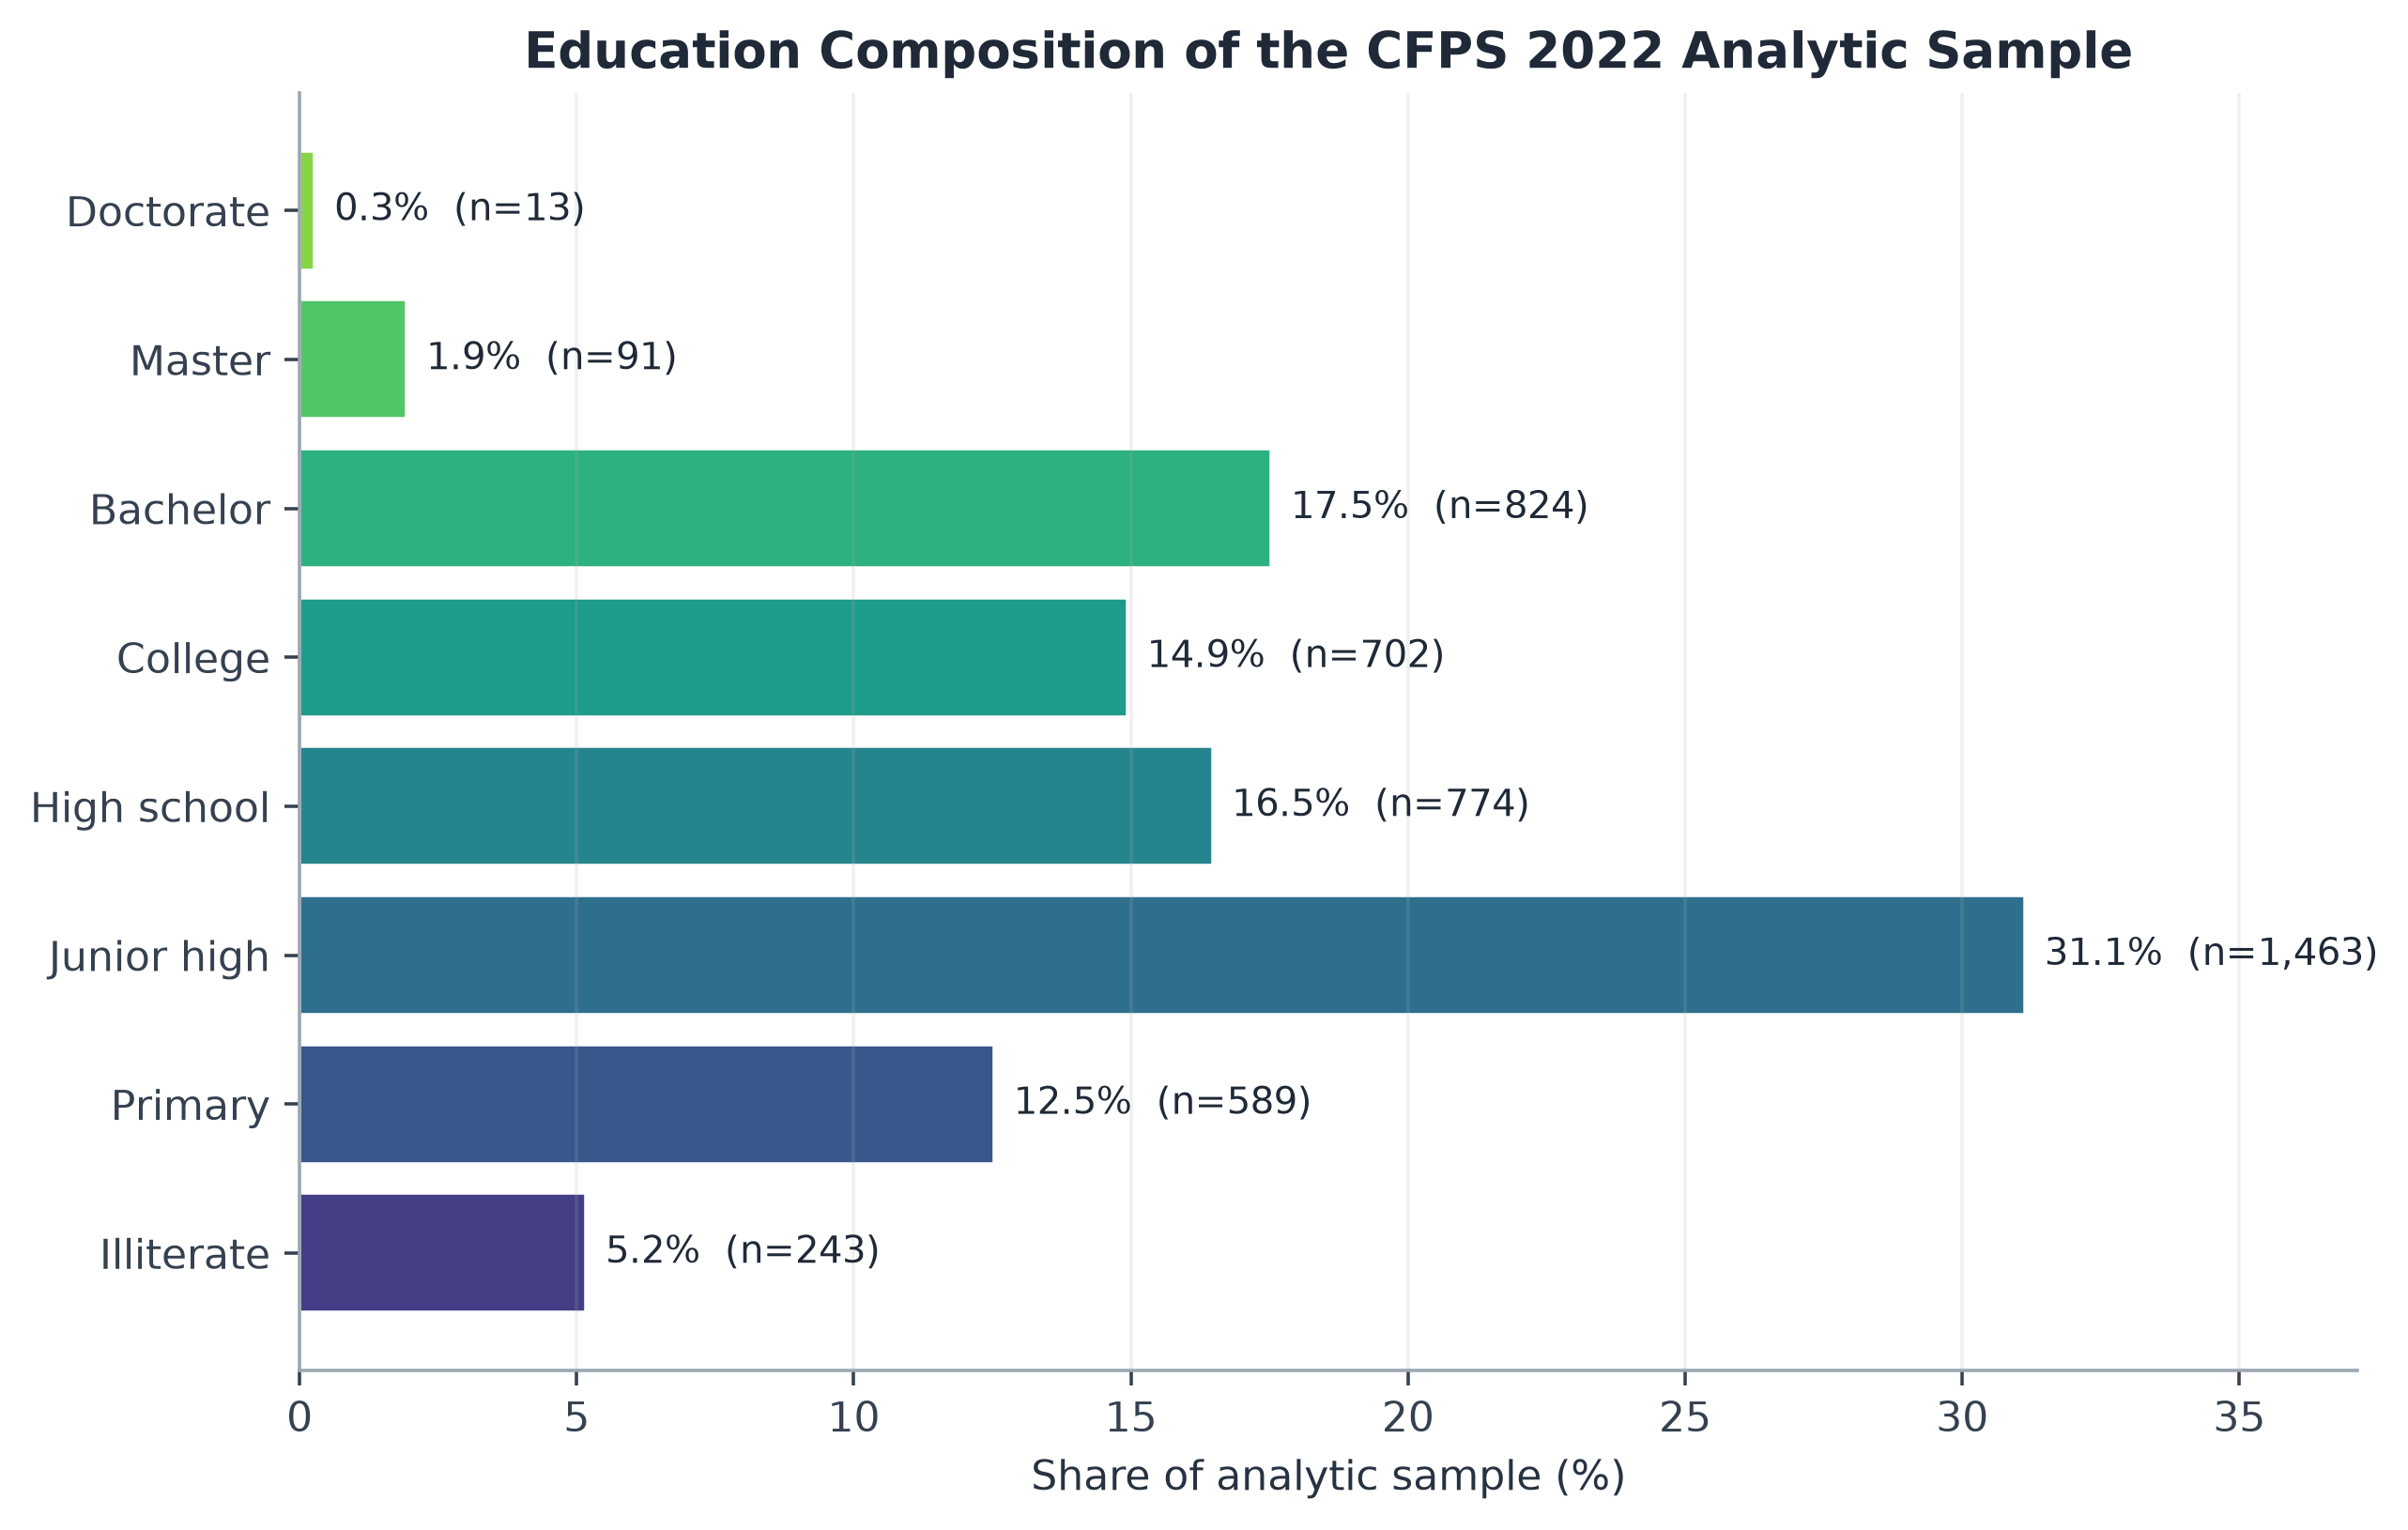
\includegraphics[width=0.86\textwidth]{figures/viz_education_distribution.png}
\caption{Education composition of the analytic sample}
\label{fig:education}
\end{figure}

\begin{figure}[H]
\centering
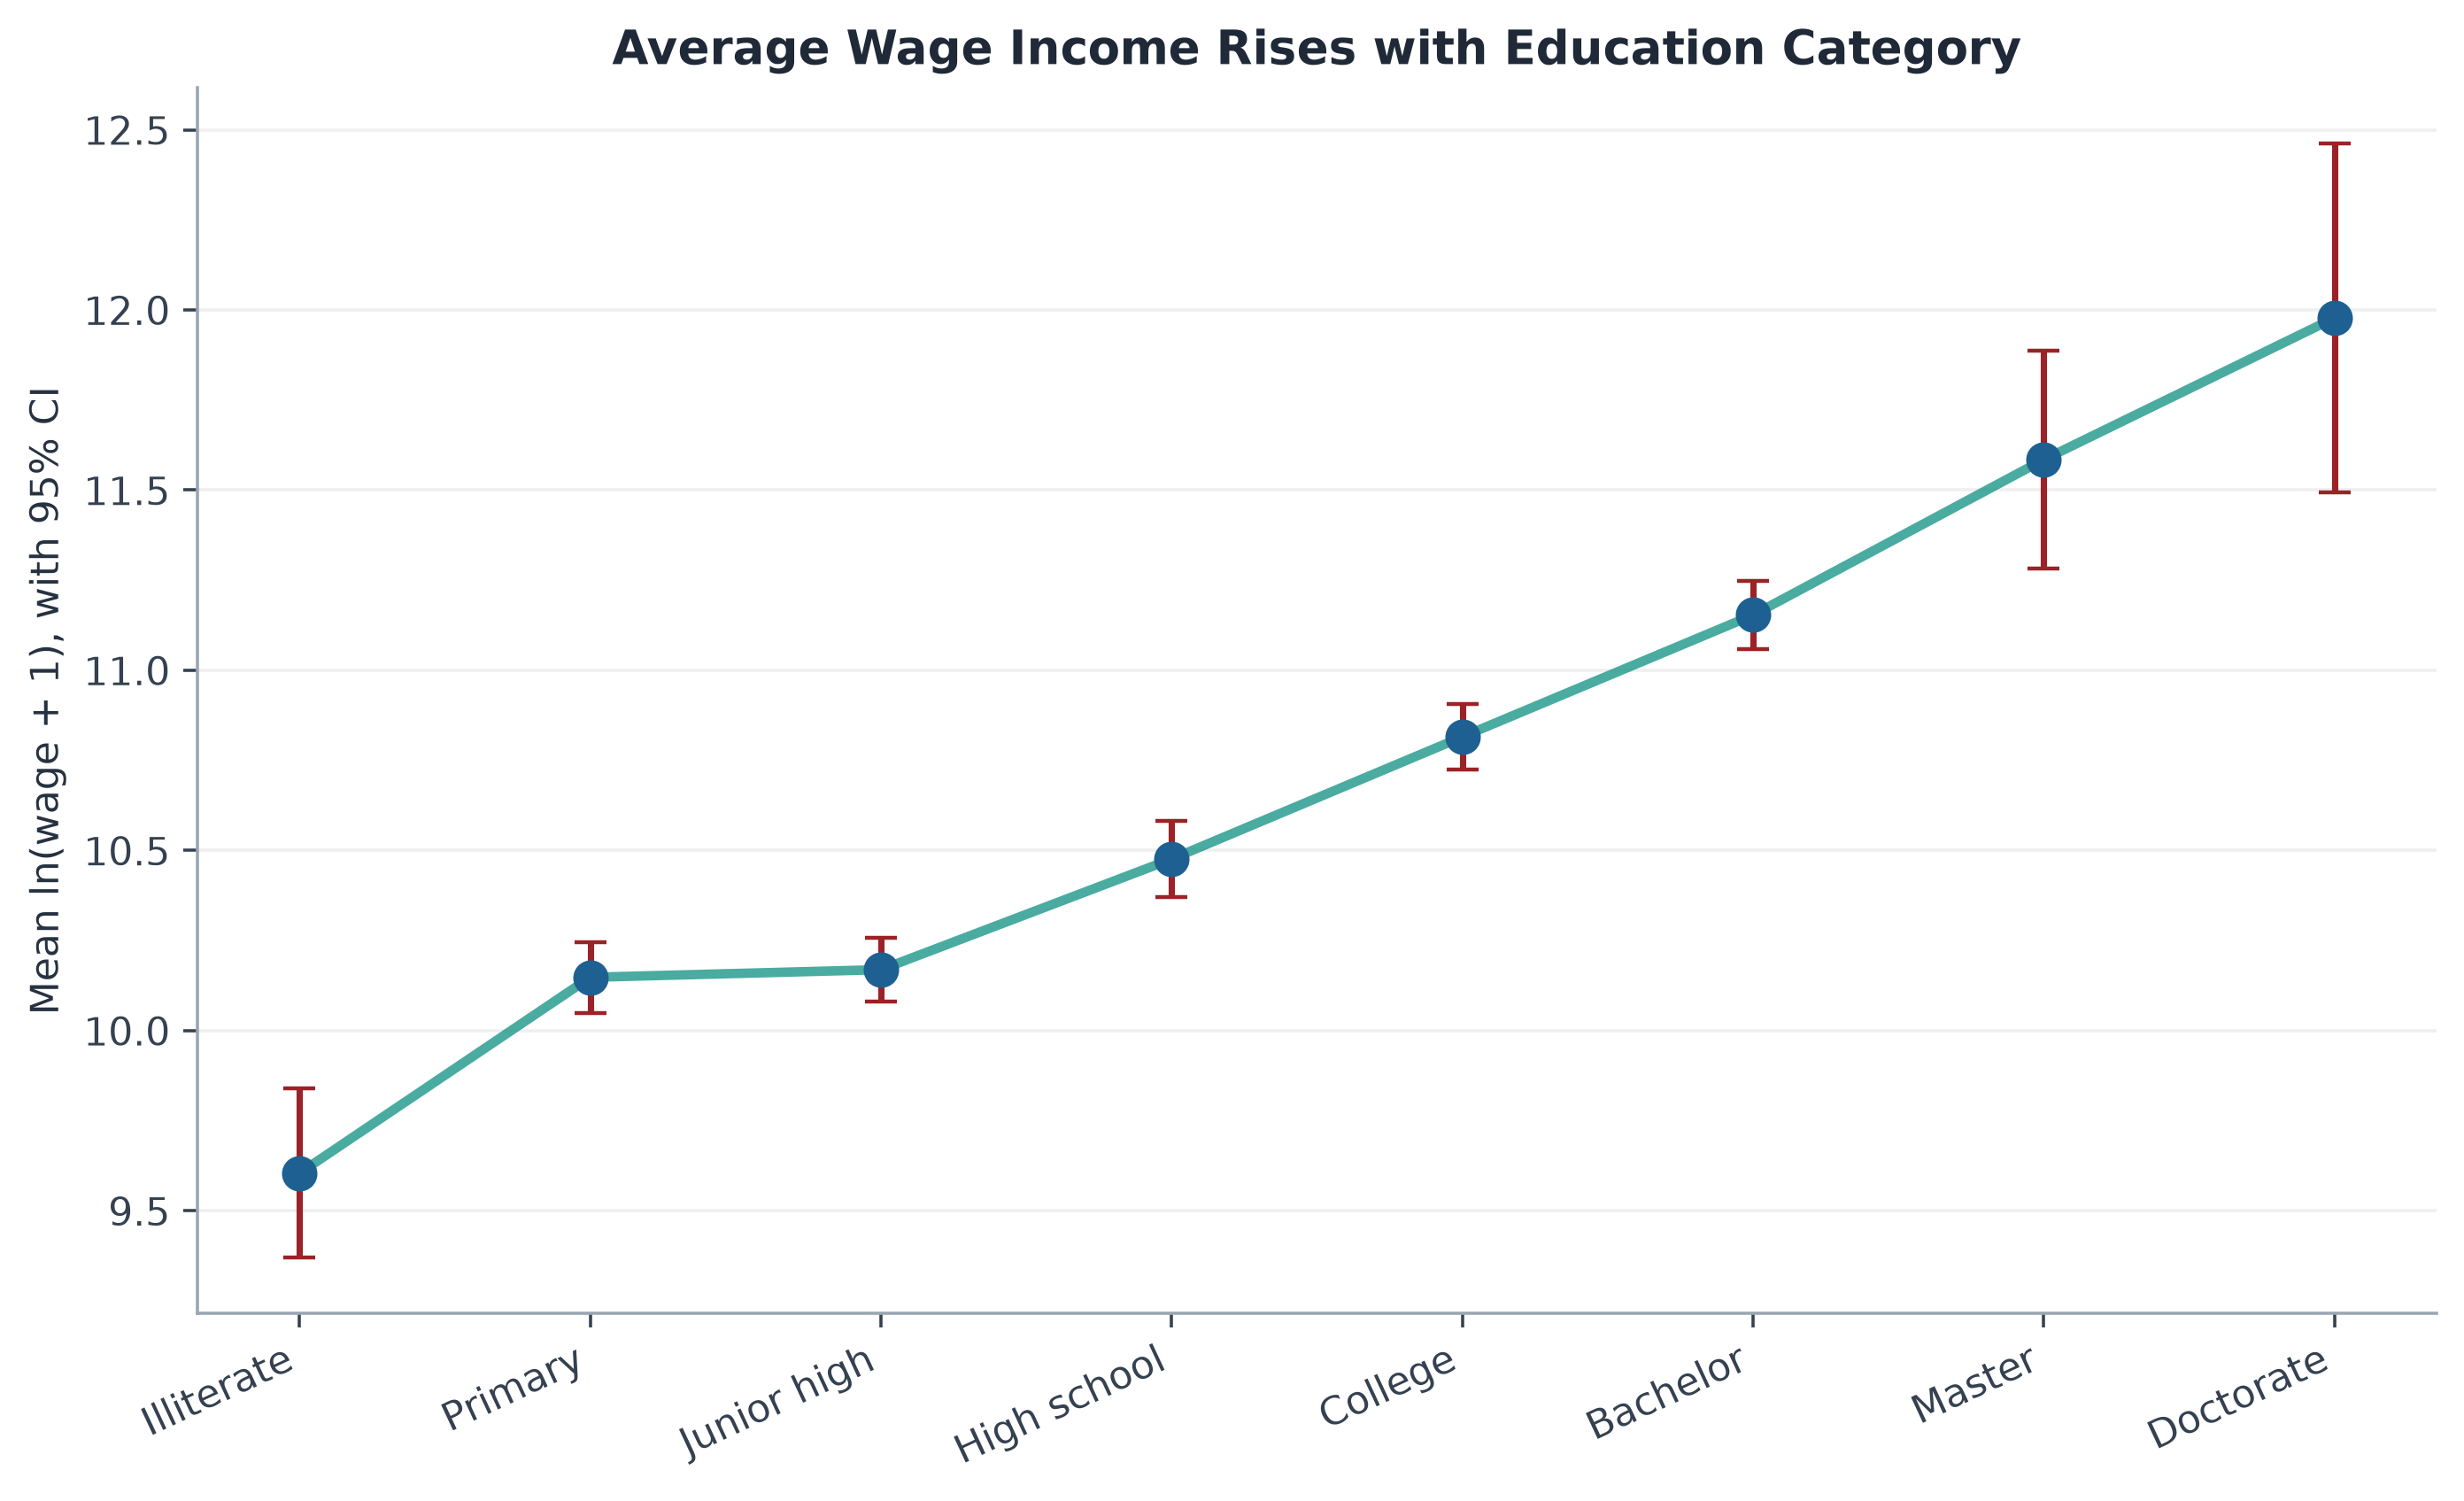
\includegraphics[width=0.86\textwidth]{figures/viz_wage_by_education.png}
\caption{Mean log wage income by education category}
\label{fig:wageedu}
\end{figure}

\section{Empirical Strategy}

\subsection{OLS Benchmark}

The benchmark model is
\begin{equation}
\ln(\mathrm{wage}_i+1)=\alpha+\beta E_i+\gamma X_i+\mu_p+\varepsilon_i,
\end{equation}
where $E_i$ is either years of schooling or college-or-above status, $X_i$ includes demographic and household controls, and $\mu_p$ denotes province fixed effects. Robust standard errors are used throughout. These regressions provide the baseline education-income gradient, but the coefficients are not interpreted as fully causal.

\subsection{Doubly Robust Treatment-Effect Estimation}

The main estimand is the average treatment effect of college-or-above education:
\begin{equation}
ATE=E[Y_i(1)-Y_i(0)].
\end{equation}
The AIPW score is
\begin{equation}
\hat{\tau}_i =
\hat{m}_1(X_i)-\hat{m}_0(X_i)
+\frac{D_i(Y_i-\hat{m}_1(X_i))}{\hat{e}(X_i)}
-\frac{(1-D_i)(Y_i-\hat{m}_0(X_i))}{1-\hat{e}(X_i)},
\end{equation}
where $D_i$ indicates college-or-above education, $\hat{e}(X_i)$ is the estimated propensity score, and $\hat{m}_d(X_i)$ is the predicted outcome under treatment status $d$. Five-fold cross-fitting is used so that the nuisance models are not trained and evaluated on exactly the same observations. The paper reports both linear and gradient-boosting nuisance models. The preferred specification uses age, gender, hukou, urban residence, marriage, medical insurance, and province. Extended specifications add health, household size, social status, internet use, and employment status as sensitivity controls.

\subsection{Expansion-Based IV Diagnostic}

China's higher-education expansion began in 1999. A natural idea is to use cohort exposure around the college-entry age as an instrument for education. The forcing variable is birth year minus 1981, because the 1981 birth cohort was approximately 18 in 1999. The diagnostic specification asks whether being born in or after 1981 creates a discontinuous increase in schooling within symmetric cohort windows. This design is useful only if the first stage is strong and local, so the first-stage coefficients and F-statistics are reported before any IV interpretation is considered.

\section{Results}

\subsection{OLS Benchmarks}

Table~\ref{tab:reg} reports the OLS benchmarks. One additional year of schooling is associated with 0.088 log points higher wage income in the basic specification and 0.083 log points in the richer specification. When education is measured as college-or-above completion, the coefficient is 0.738 in the basic specification and 0.694 with richer controls. The estimates remain positive across definitions of education and income, suggesting that the education-income gradient is not an artifact of one particular specification.

\begin{table}[H]
\centering
\caption{OLS Benchmark Estimates}
\label{tab:reg}
\begin{tabular}{lrrrr}
\toprule
Specification & Coefficient & Robust SE & N & $R^2$ \\
\midrule
Years, basic controls & 0.0882*** & (0.0060) & 4,699 & 0.158 \\
Years, rich controls & 0.0824*** & (0.0063) & 4,637 & 0.163 \\
College, basic controls & 0.7405*** & (0.0488) & 4,699 & 0.153 \\
College, rich controls & 0.6949*** & (0.0497) & 4,637 & 0.162 \\
Winsorized wage & 0.7317*** & (0.0485) & 4,699 & 0.152 \\
Positive wage only & 0.6438*** & (0.0294) & 4,638 & 0.285 \\
\bottomrule
\end{tabular}

\begin{flushleft}
\footnotesize Notes: Robust standard errors are in parentheses. Basic controls include age, age squared, gender, marriage, rural hukou, medical insurance, and province fixed effects. Rich controls additionally include urban residence, health, household size, internet use, and subjective social status. $^{*}p<0.10$, $^{**}p<0.05$, $^{***}p<0.01$.
\end{flushleft}
\end{table}

\begin{figure}[H]
\centering
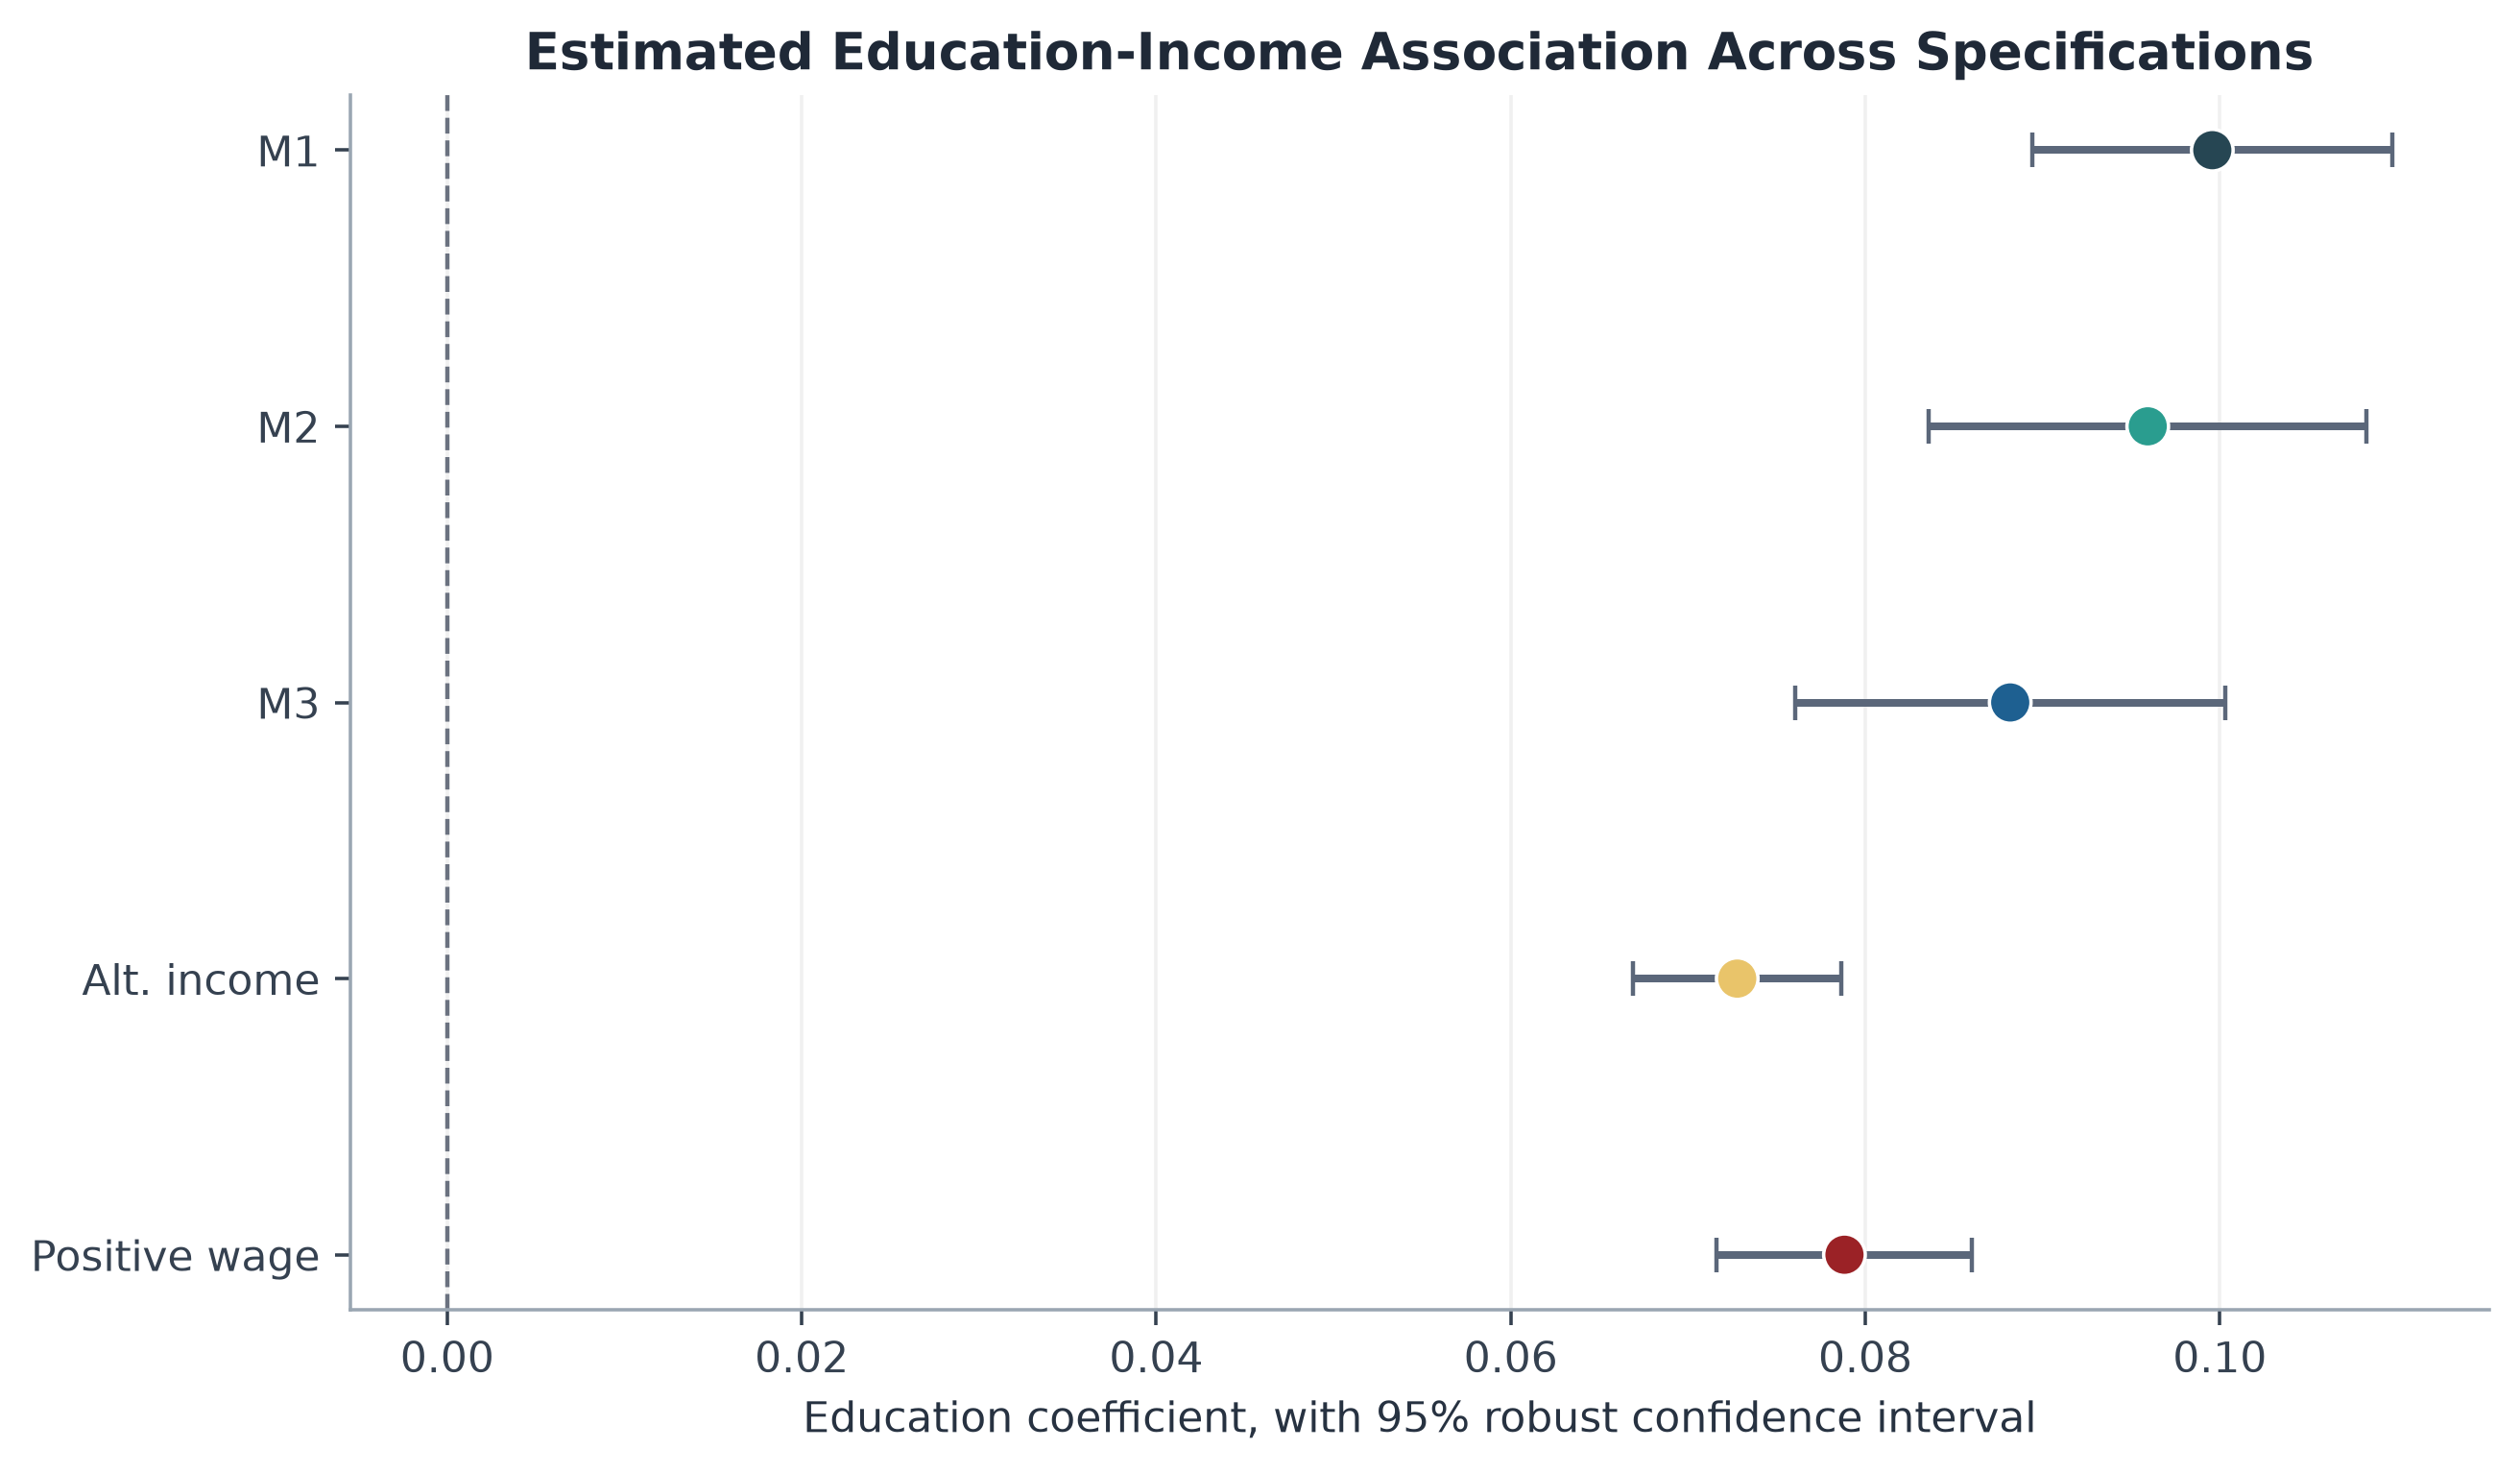
\includegraphics[width=0.86\textwidth]{figures/viz_regression_coefficients.png}
\caption{Regression coefficients across specifications}
\label{fig:coef}
\end{figure}

\subsection{Doubly Robust Estimates}

Table~\ref{tab:aipw} reports the AIPW results. The preferred core-plus GBM estimate is 0.710 log points with a standard error of 0.056. Across six specifications, estimates range from 0.669 to 0.773 log points. These estimates are slightly smaller than the OLS college coefficient but still large, which suggests that the college-income premium remains visible after balancing observed differences between the two education groups.

\begin{table}[H]
\centering
\caption{AIPW Estimates for College-or-Above Education}
\label{tab:aipw}
\input{tables/table_aipw_effects.tex}
\begin{flushleft}
\footnotesize Notes: The outcome is $\ln(\mathrm{wage}+1)$. ATE is the estimated average treatment effect of completing college or above. Linear uses logistic/Ridge nuisance models; GBM uses gradient boosting. The preferred specification is Core plus with GBM.
\end{flushleft}
\end{table}

The credibility of AIPW depends on overlap and balance. Figure~\ref{fig:propensity} shows that treatment and control units share a broad common propensity-score region, although a small number of observations lie near the tails. Those tails are a reminder that the estimate is not free of extrapolation risk. Table~\ref{tab:balance} and Figure~\ref{fig:balance} show that weighting reduces absolute standardized differences for core covariates to below 0.10.

\begin{figure}[H]
\centering
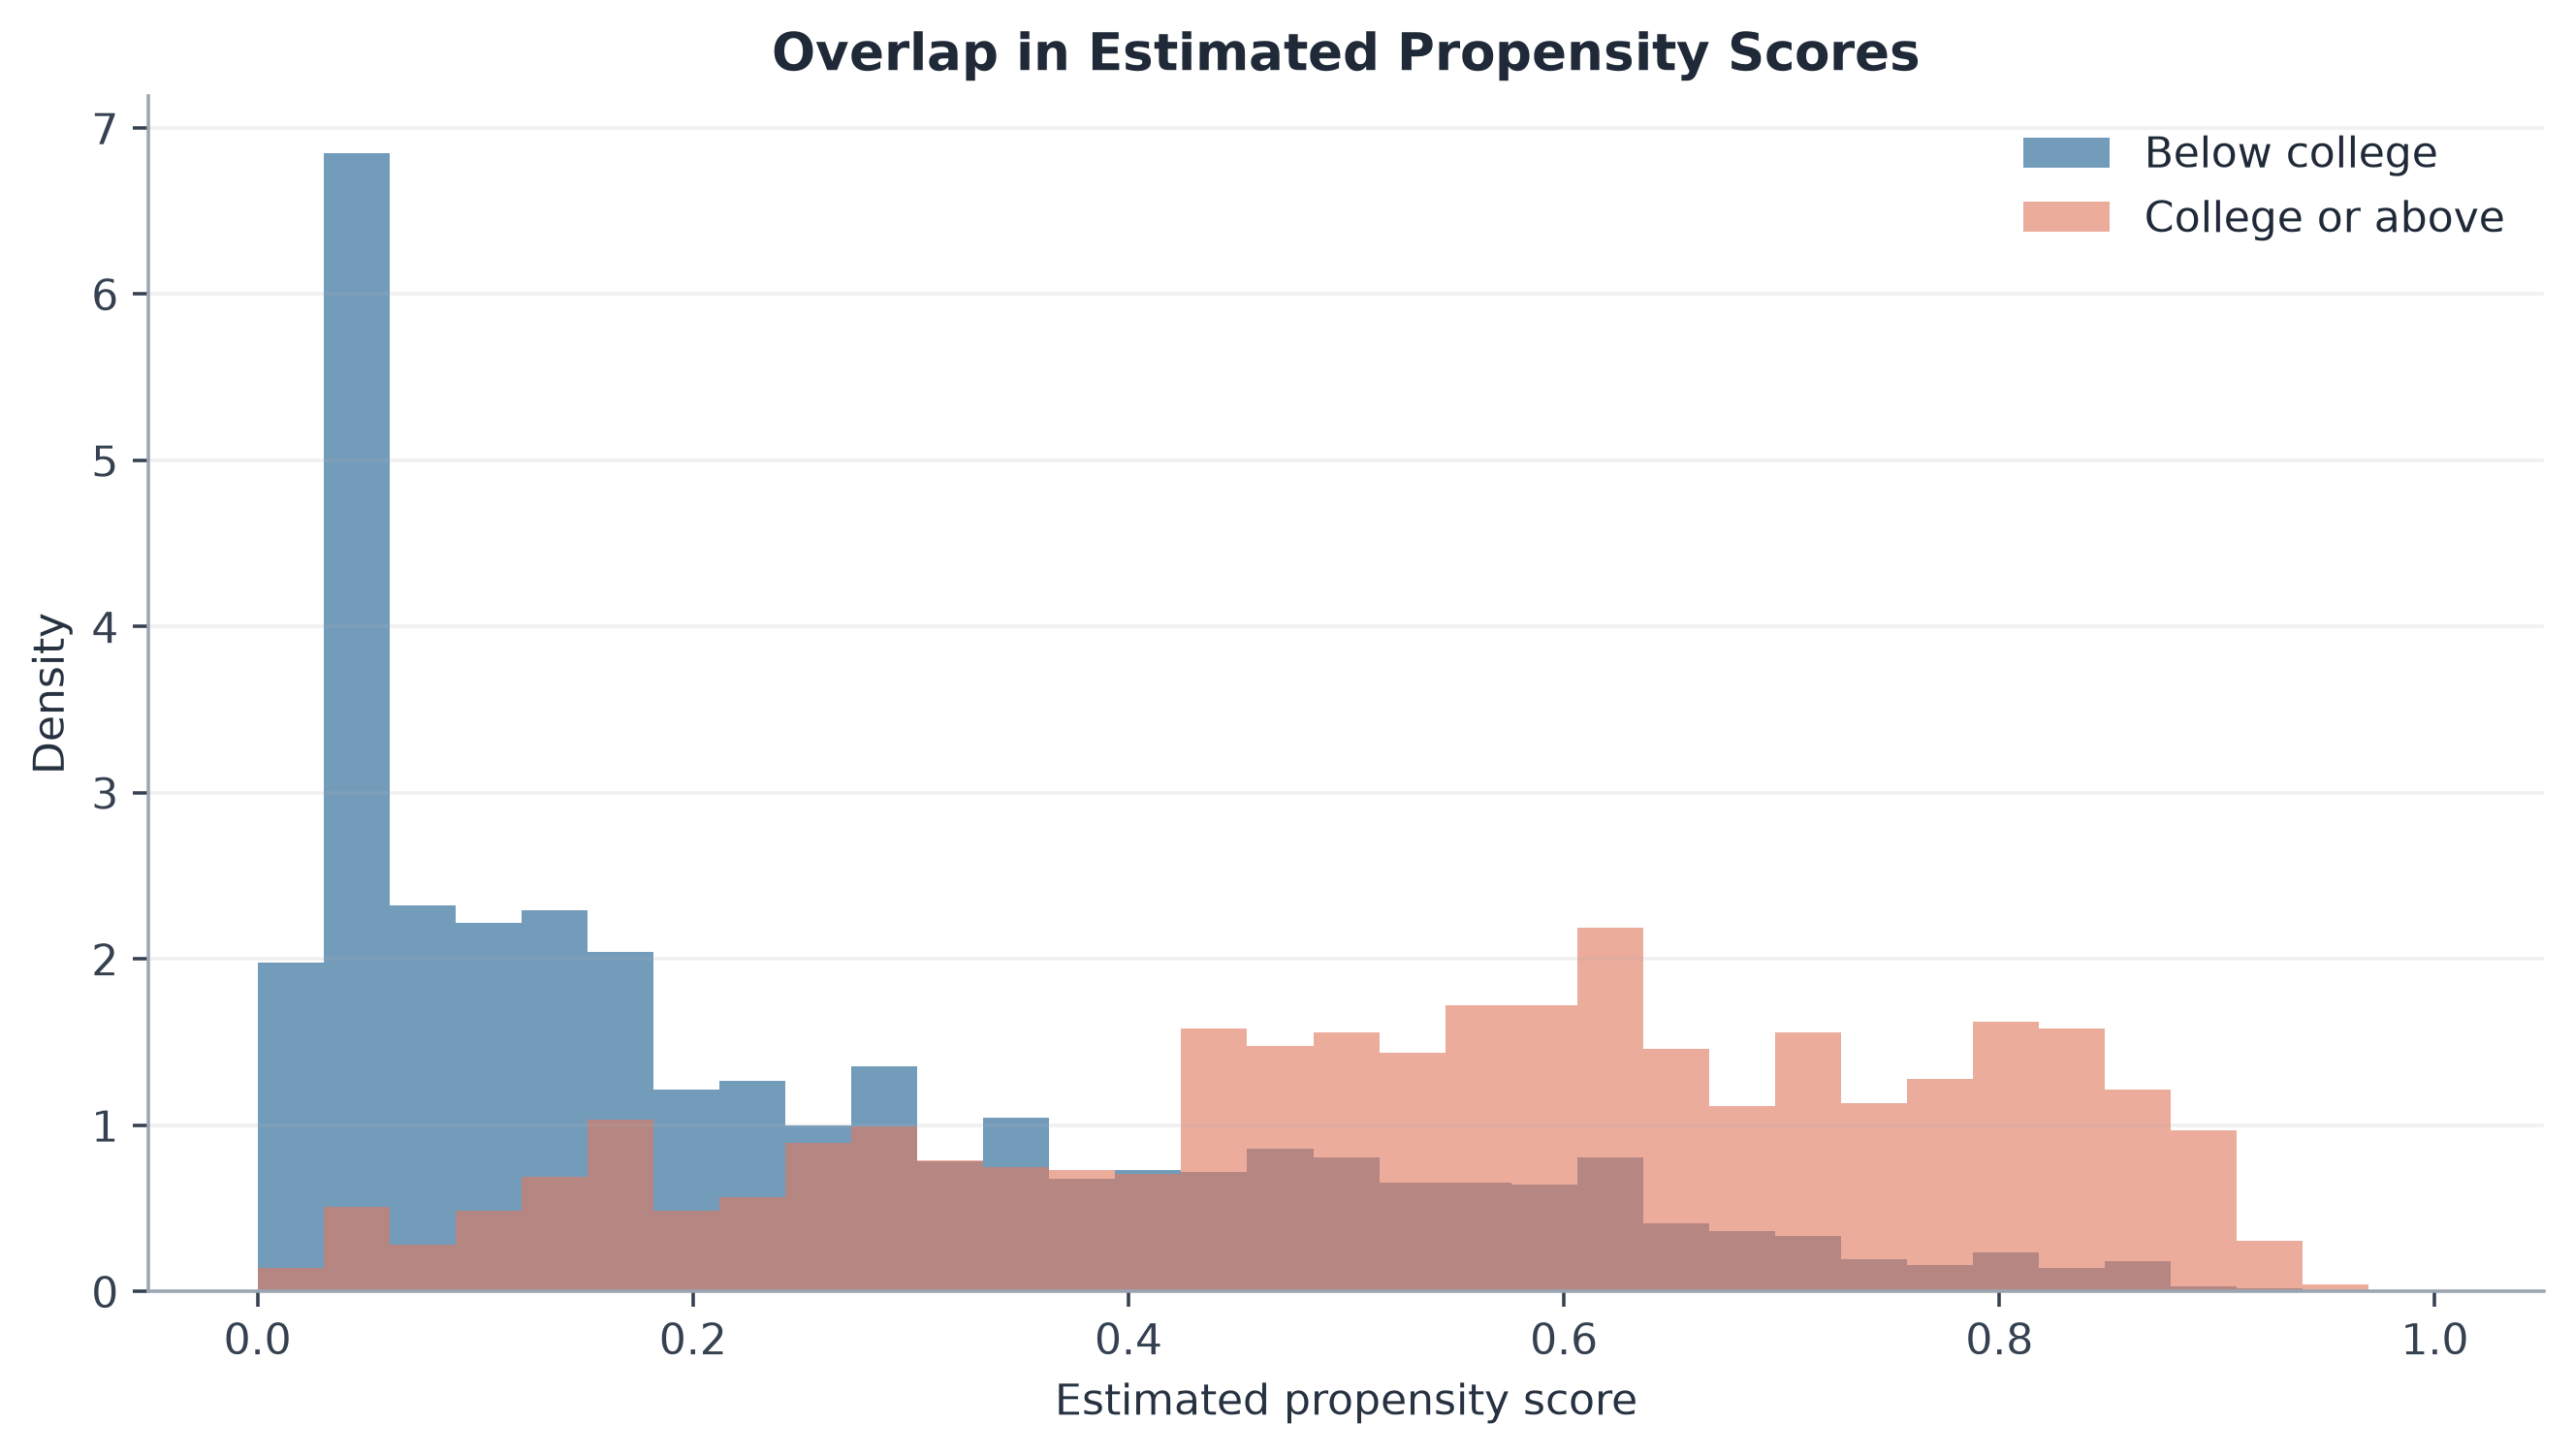
\includegraphics[width=0.86\textwidth]{figures/viz_propensity_overlap.png}
\caption{Propensity-score overlap}
\label{fig:propensity}
\end{figure}

\begin{table}[H]
\centering
\caption{Covariate Balance Before and After Weighting}
\label{tab:balance}
\begin{tabular}{lrr}
\toprule
Covariate & Raw SMD & Weighted SMD \\
\midrule
age\_ & -0.937 & -0.072 \\
gen & -0.214 & 0.033 \\
rural & -0.525 & -0.024 \\
urban & 0.642 & 0.033 \\
mar & -0.286 & -0.023 \\
medsure\_dum & 0.079 & -0.001 \\
\bottomrule
\end{tabular}

\end{table}

\begin{figure}[H]
\centering
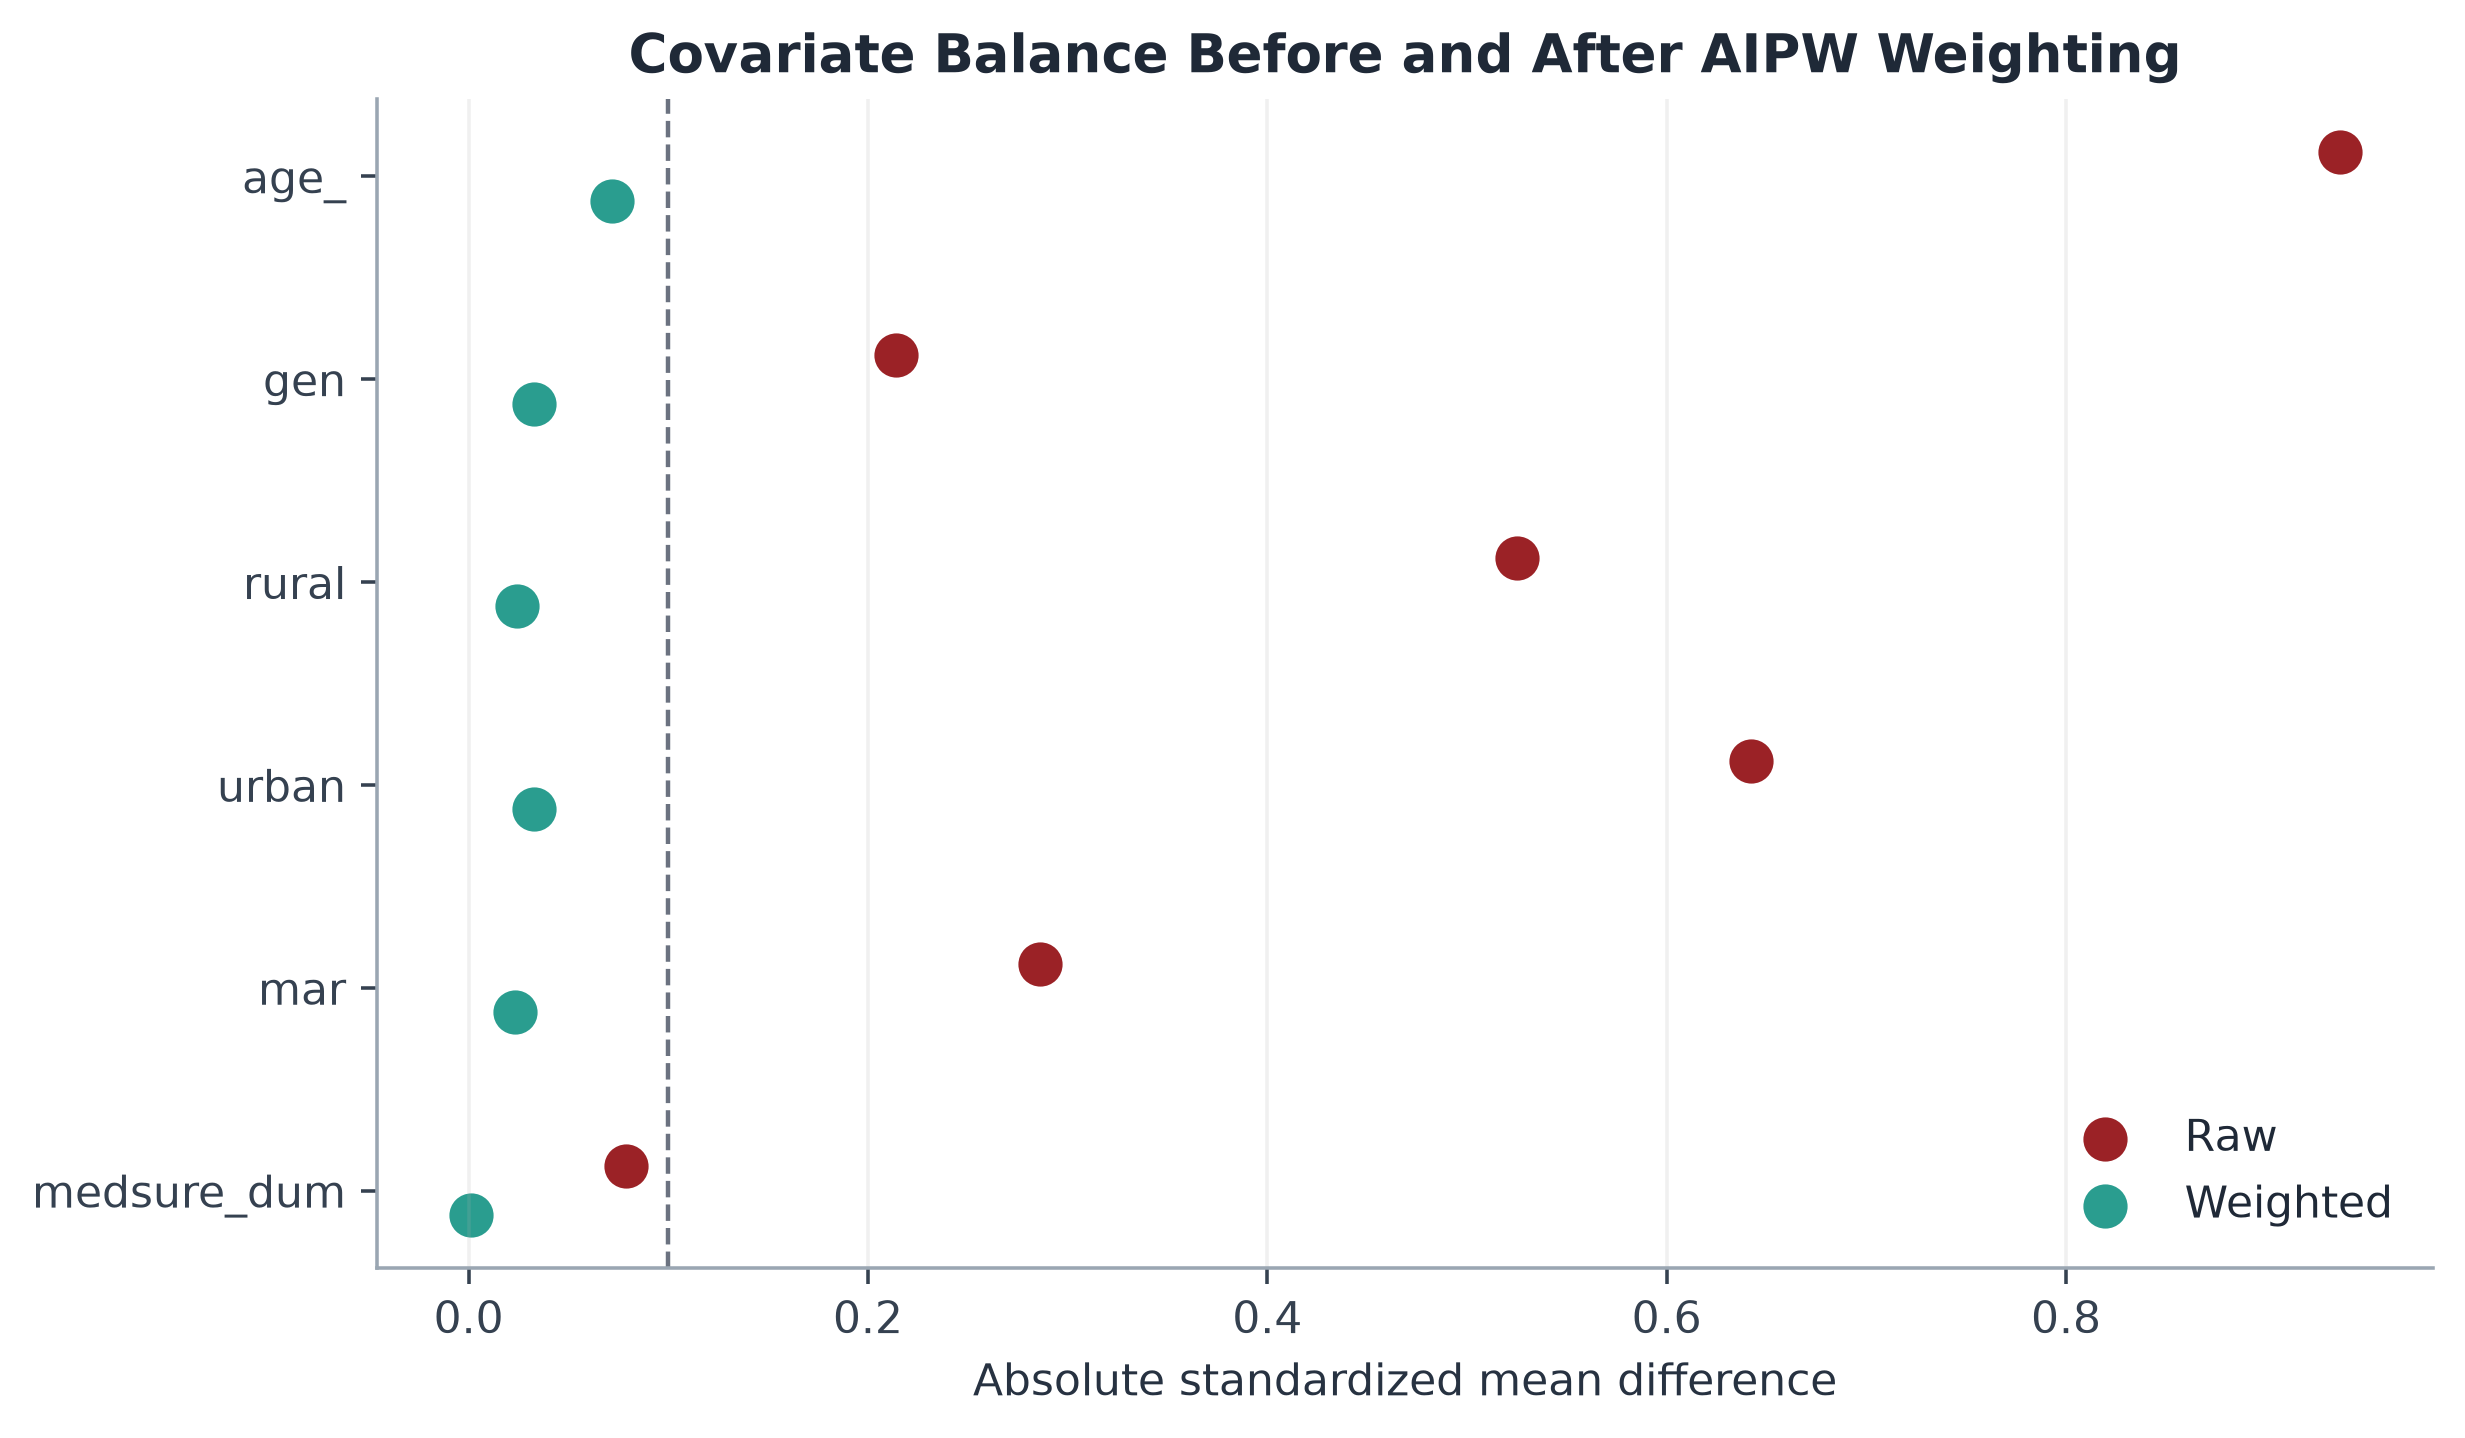
\includegraphics[width=0.80\textwidth]{figures/viz_balance_diagnostics.png}
\caption{Standardized mean differences before and after weighting}
\label{fig:balance}
\end{figure}

\subsection{Weak-IV Diagnostic}

Figure~\ref{fig:cohort} plots college completion and average schooling by birth cohort around the 1981 cutoff. Table~\ref{tab:iv} reports the formal first-stage and IV diagnostics. In narrow windows of $\pm 5$ to $\pm 15$ years, the first-stage F-statistics are far below conventional weak-instrument thresholds. The $\pm 20$ window has a strong first stage, but it is too wide to read as a local discontinuity because it spans a broad range of cohorts and life-cycle positions. The policy-based IV design is therefore reported as a checked but unsuccessful identification route, not as the main causal estimate.

\begin{figure}[H]
\centering
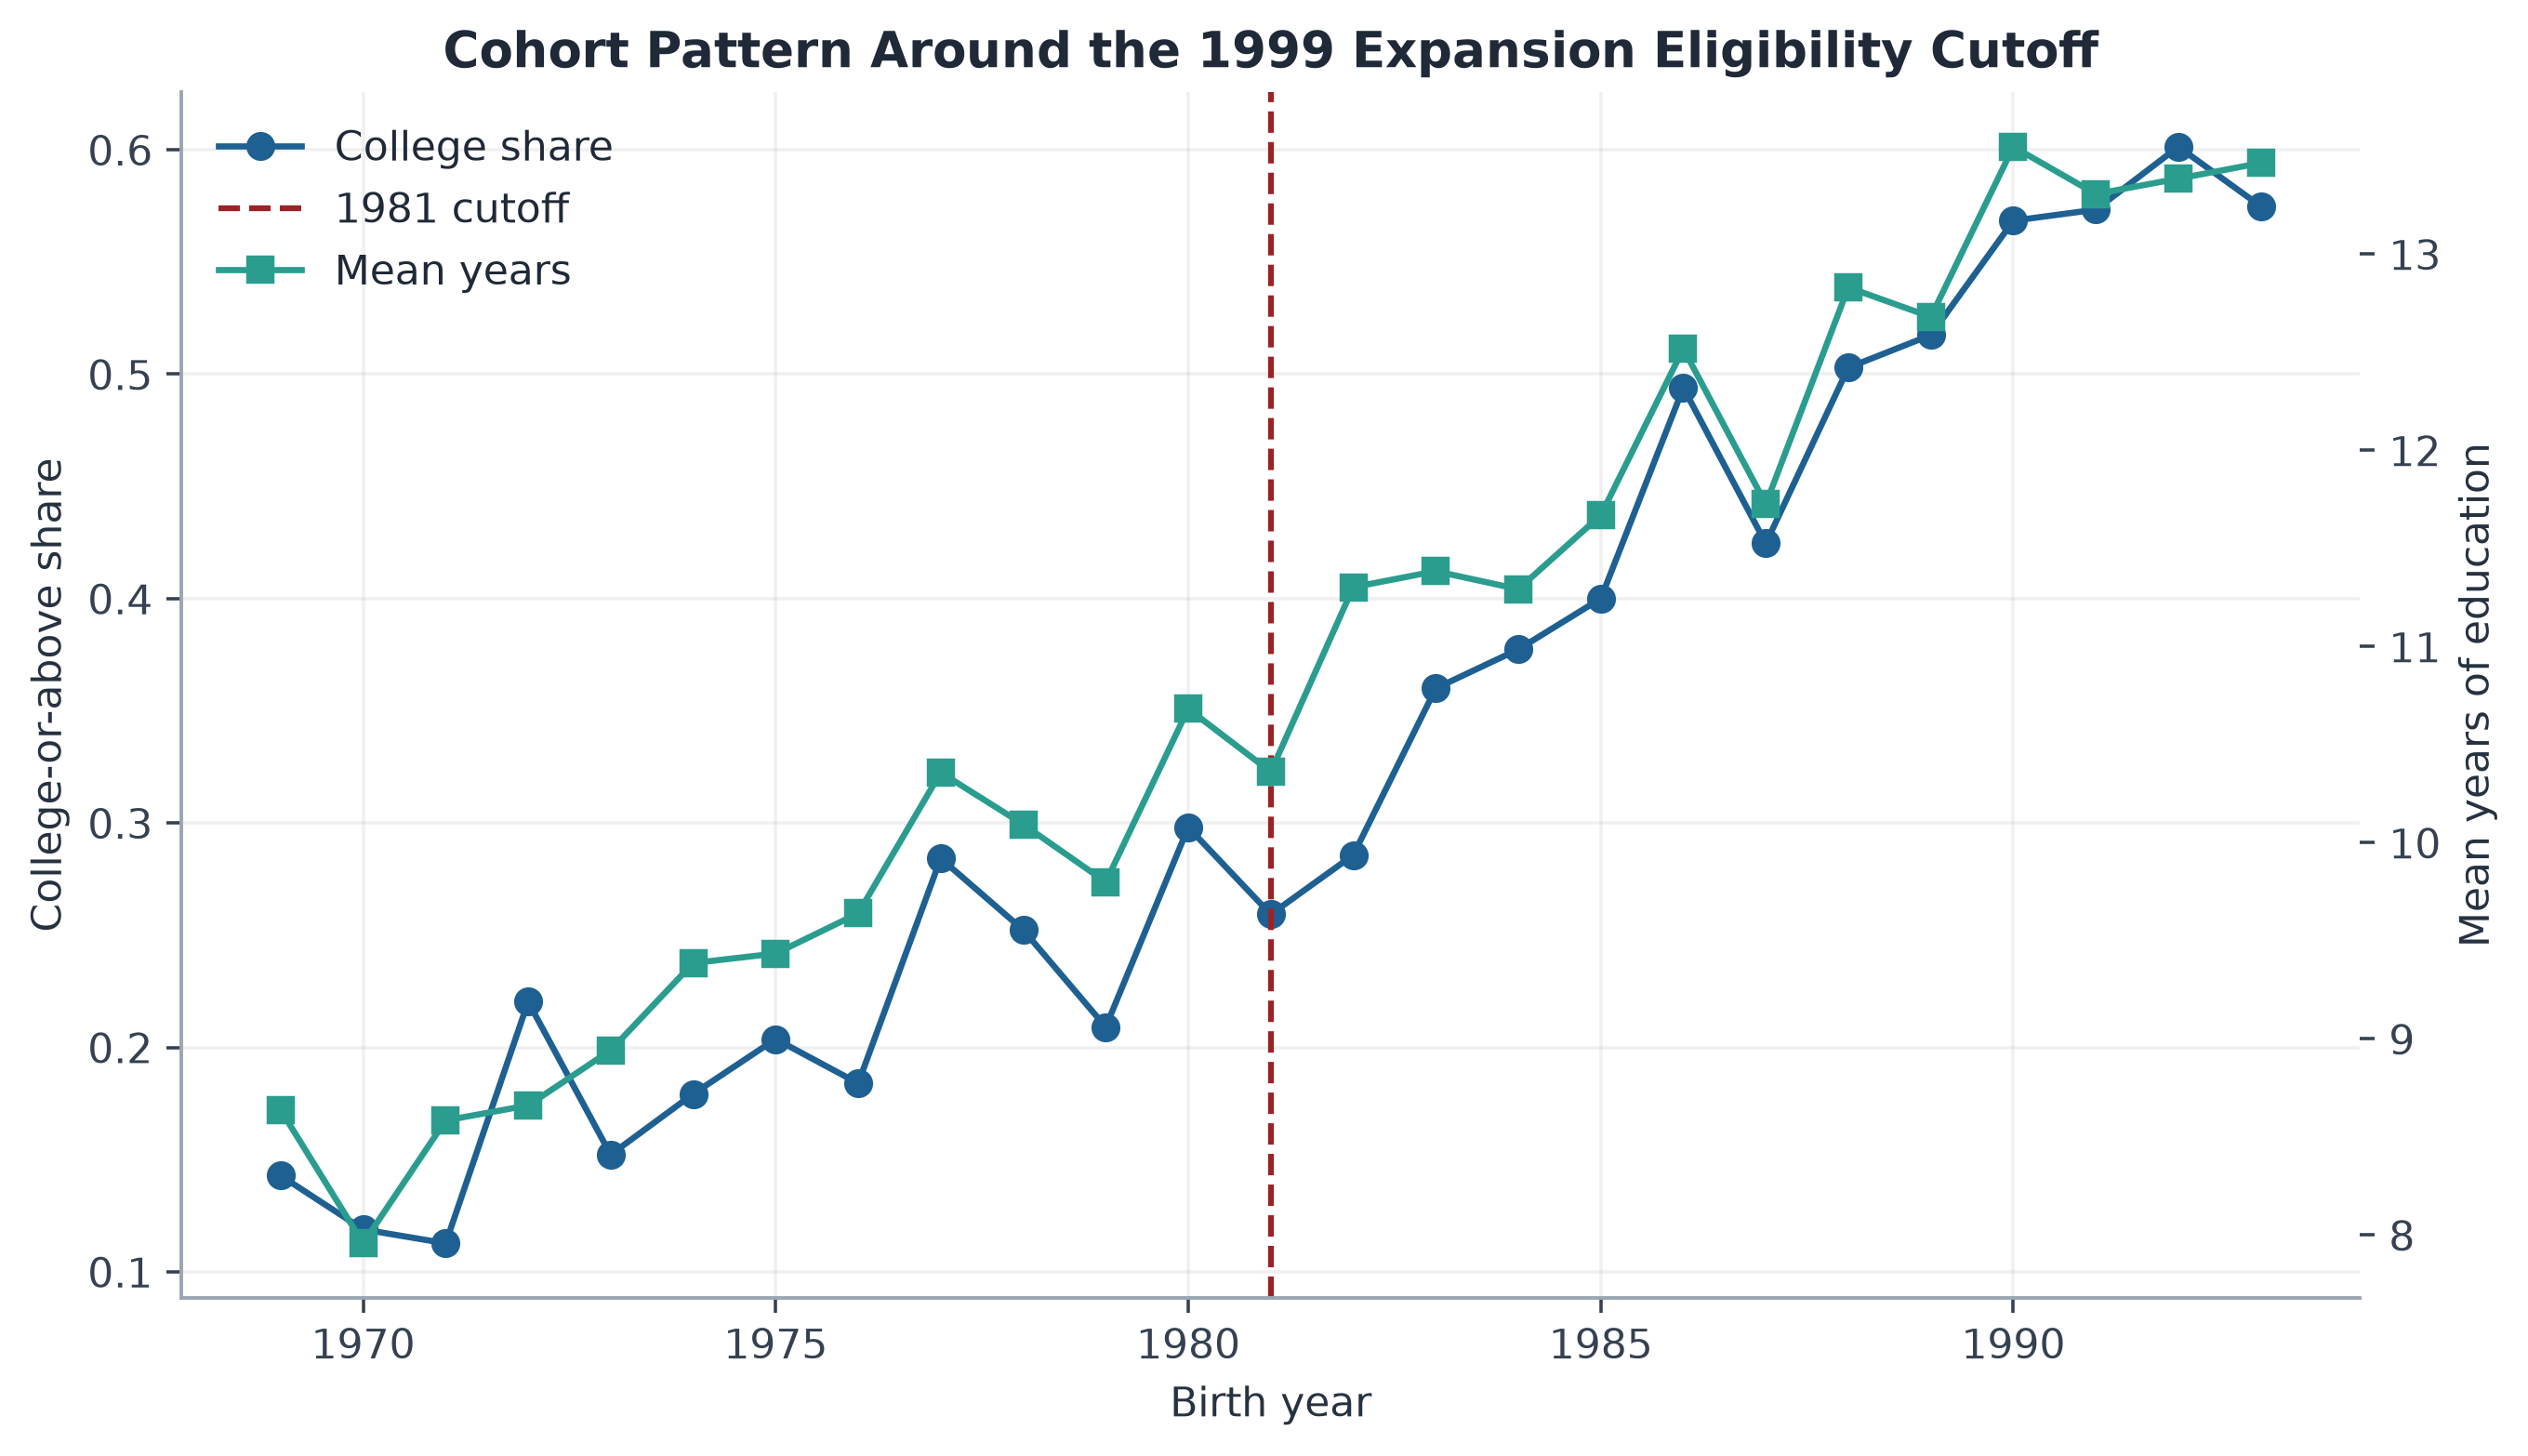
\includegraphics[width=0.86\textwidth]{figures/viz_cohort_first_stage.png}
\caption{Cohort pattern around the expansion eligibility cutoff}
\label{fig:cohort}
\end{figure}

\begin{table}[H]
\centering
\caption{Higher-Education Expansion IV Diagnostics}
\label{tab:iv}
\begin{tabular}{lrrrrr}
\toprule
Window & N & First stage & F-stat & IV estimate & SE \\
\midrule
+/-5 & 1,280 & -0.0743 & 0.03 & 0.5195 & (3.2703) \\
+/-7 & 1,844 & 0.1961 & 0.29 & 0.4589 & (0.9572) \\
+/-9 & 2,462 & -0.0481 & 0.02 & 0.2091 & (2.4996) \\
+/-12 & 3,277 & 0.1269 & 0.21 & -0.7816 & (2.0357) \\
+/-15 & 3,933 & 0.3977 & 2.54 & -0.1531 & (0.2721) \\
+/-20 & 4,596 & 1.2985 & 33.22 & 0.0414 & (0.0633) \\
\bottomrule
\end{tabular}

\begin{flushleft}
\footnotesize Notes: The instrument is an indicator for birth year 1981 or later, with linear running variable controls and province fixed effects. The weak first stage in narrow windows means the IV results should not be read as the main causal evidence.
\end{flushleft}
\end{table}

\subsection{Heterogeneity}

Education-income associations are stronger for women than men and stronger for non-rural hukou holders than rural hukou holders. This is consistent with recent evidence that education returns in China vary by gender, hukou, sector, and region \citep{ma2021meta, li2025gender}.

\begin{table}[H]
\centering
\caption{Heterogeneous Education Coefficients}
\label{tab:heterogeneity}
\begin{tabular}{lrrrr}
\toprule
Subsample & Education coefficient & Robust SE & N & $R^2$ \\
\midrule
Women & 0.1104*** & (0.0094) & 1,996 & 0.155 \\
Men & 0.0668*** & (0.0069) & 2,703 & 0.145 \\
Non-rural hukou & 0.1482*** & (0.0201) & 962 & 0.144 \\
Rural hukou & 0.0771*** & (0.0066) & 3,737 & 0.128 \\
\bottomrule
\end{tabular}

\end{table}

\begin{figure}[H]
\centering
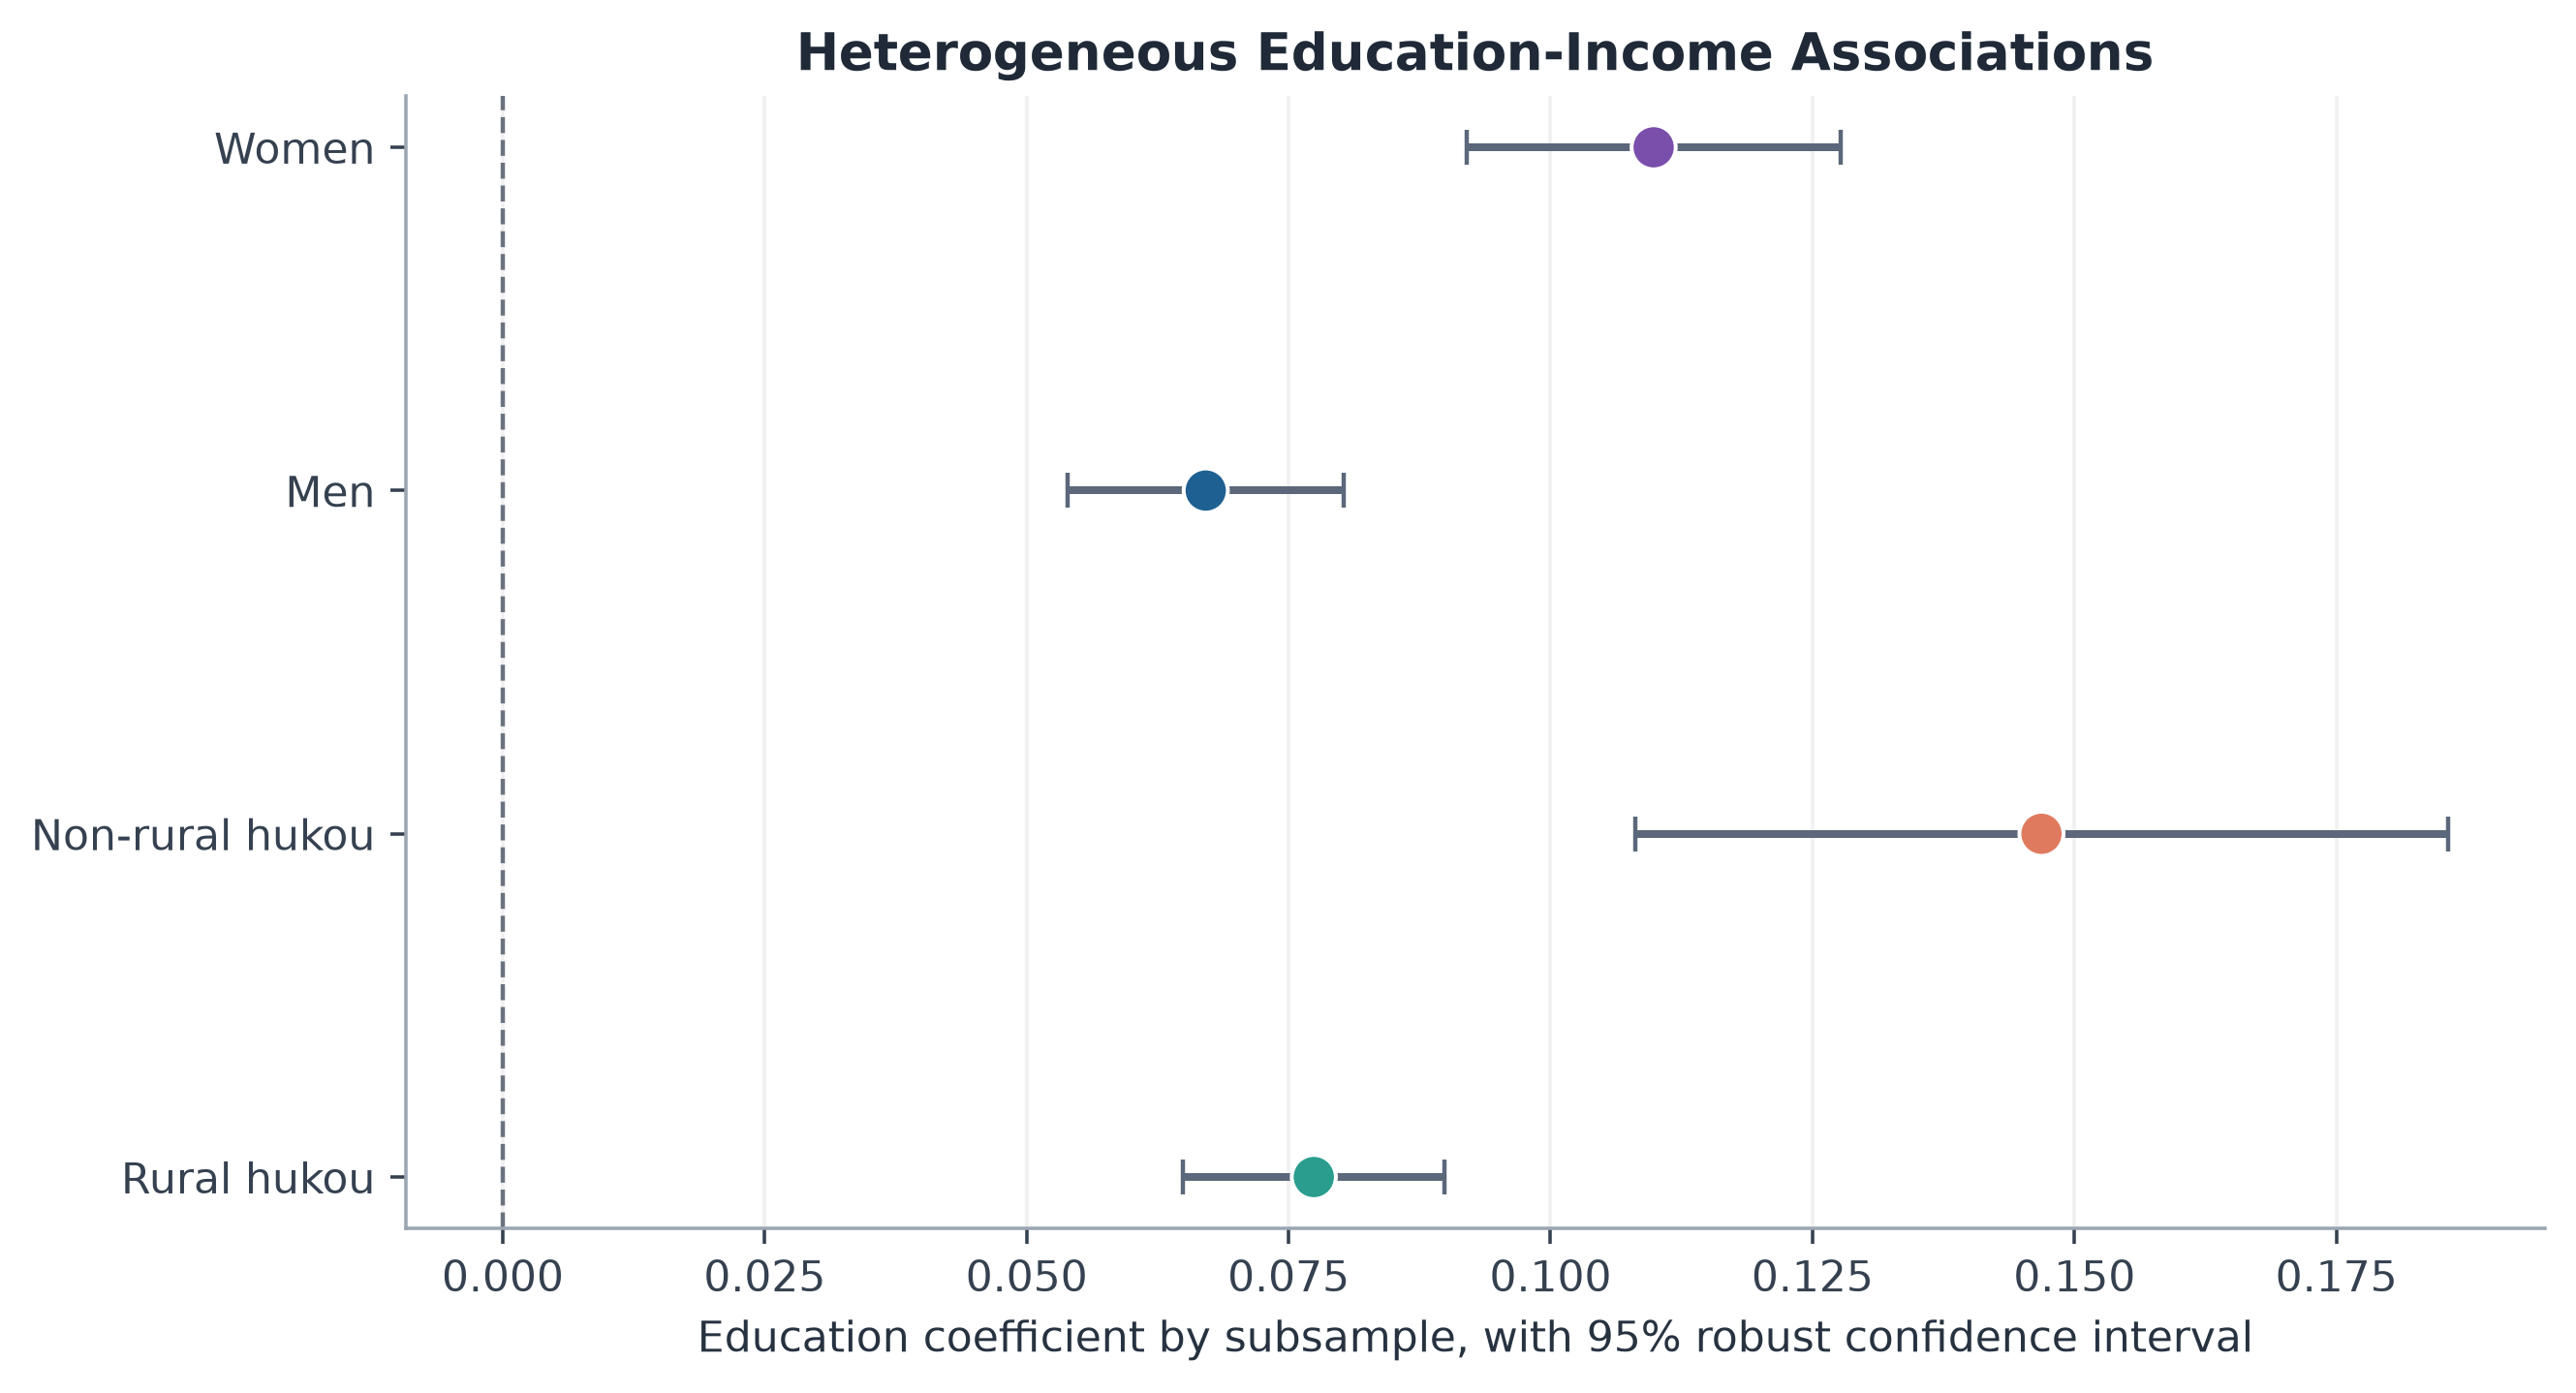
\includegraphics[width=0.82\textwidth]{figures/viz_heterogeneity_coefficients.png}
\caption{Education-income association by gender and hukou subsample}
\label{fig:heterogeneity}
\end{figure}

\section{Discussion}

The results should be read as a set of checks rather than as a single coefficient. The sample audit shows where observations are lost and how the wage tail is handled. The OLS models establish the baseline education-income gradient. The AIPW estimates show that the college-income gap remains large after balancing observed characteristics. The expansion diagnostic, meanwhile, shows that the current cross-section does not provide a strong local IV design. This combination gives a clearer empirical story than a standalone significant education coefficient.

The main limitation is that AIPW still depends on observed covariates. CFPS 2022 lacks direct measures of ability, parental education in the working file, school quality, and childhood family resources. Therefore, the preferred estimate should be interpreted as a selection-on-observables treatment-effect estimate, not as a definitive natural-experiment estimate. The weak-IV diagnostic also shows why it would be misleading to claim a strong expansion-based causal result from this cross-section alone.

\section{Conclusion}

Using CFPS 2022, this paper finds a large positive education-income relationship among Chinese adults. The conventional Mincer coefficient is about 0.088 per year of schooling. In the AIPW framework, completing college or above is associated with roughly 0.71 log points higher wage income after balancing observed covariates. The estimate is stable across alternative nuisance models and covariate sets, and the balance diagnostics improve after weighting. A cautious reading is that, within the limits of the observed data, higher education remains closely linked to higher wages. Stronger causal claims would require a cleaner policy shock, panel evidence, or richer measures of family background and ability.

\bibliographystyle{plainnat}
\bibliography{references}

\end{document}
